\documentclass[11pt,psfig]{article}
\usepackage{epsfig}
\usepackage{times}
\usepackage{amssymb}
\usepackage{float}

\newcount\refno\refno=1
\def\ref{\the\refno \global\advance\refno by 1}
\def\ux{\underline{x}}
\def\uw{\underline{w}}
\def\bw{\underline{w}}
\def\ut{\underline{\theta}}
\def\umu{\underline{\mu}} 
\def\bmu{\underline{\mu}} 
\def\be{p_e^*}
\newcount\eqnumber\eqnumber=1
\def\eq{\the \eqnumber \global\advance\eqnumber by 1}
\def\eqs{\eq}
\def\eqn{\eqno(\eq)}

 \pagestyle{empty}
\def\baselinestretch{1.1}
\topmargin1in \headsep0.3in
\topmargin0in \oddsidemargin0in \textwidth6.5in \textheight8.5in
\begin{document}
\setlength{\parskip}{1.2ex plus0.3ex minus 0.3ex}


\thispagestyle{empty} \pagestyle{myheadings} \markright{G}



\title{CS 266 Homework 6}
\author{Zachary DeStefano, PhD Student, 15247592}
\date{Due Date: May 22}

\maketitle

\vfill\eject

\section*{Problem 6.13}

As a vertical line sweeps across, it will be making a trapezoid. \\
At a left endpoint, there are three trapezoids:\\
1. One already existing to the left of the new segment\\
2. One being made above existing segment to the right\\
3. One being made below existing segment to the right\\
\\
At a right endpoint, there are three trapezoids:\\
1. One already existing to the left above the old segment\\
2. One alright existing to the left below the old segment\\
3. One being made to the right of the old segment\\
\\
There are n segments that have left and right endpoints and at a left endpoint, there are 2 being made while at the right endpoint, there is one being made, thus for each segment, 3 trapezoids are made. With the very first endpoint though, 4 trapezoids are made because there is not one already existing to the left and it has to be made. Thus there are at most $3n+1$ trapezoids. 

\section*{Problem 6.15}

Divide the sphere into cross-sections by y-coordinate. Equivalently, it can also be divided into strips by angle from the origin. The top and bottom strips would have a degenerate side. \\
\\
Each strip will have a side on top and a side on the bottom that are both circles centered on the y-axis. You will then partition the strip by angle from the y-axis. An arc will be drawn from the top to bottom circle if the angle $\theta$ that the endpoints of the arc make with the y-axis matches. \\
\\
You can use this as a point location data structure. You will start with the surface of the sphere and then continue to divide it up using the method described above and you will eventually obtain a History DAG as required. Let $\phi$ be the angle from the origin and $\theta$ be the angle to the y-axis. To get the corresponding patch given a point on the sphere, you will find $\phi$ and $\theta$ for the point and traverse the history DAG until you get to the desired patch. \\

\newpage

\section*{Problem 12.4}

If we have a set of segments such that each line will split at least one other segment, then the auto-partitions could have more nodes in the trees than the least possible partition. \\
\\
Here is an example of 3 line segments to partition:
\begin{figure}[H]
\centering
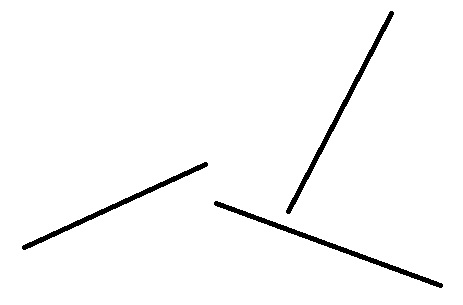
\includegraphics[height=3in]{hw6prob3diagram1.jpg}
\caption{Set of Line Segments to Partition}
\end{figure}
\newpage
Here is a binary space partition that uses only 3 segments:
\begin{figure}[H]
\centering
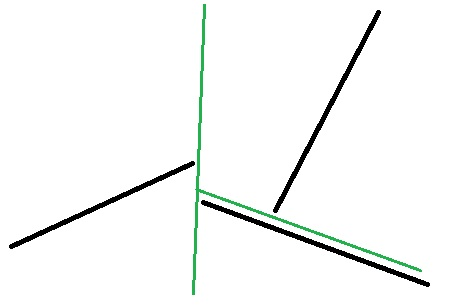
\includegraphics[height=3in]{hw6prob3diagram2.jpg}
\caption{Set of Line Segments Partitioned using the green lines}
\end{figure}

Each auto-partition will split up another line, thus at least 4 nodes are needed for an auto-partition, as can be seen with this example one
\begin{figure}[H]
\centering
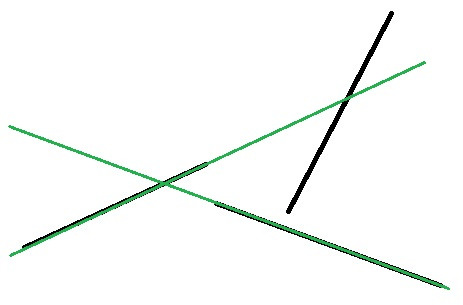
\includegraphics[height=3in]{hw6prob3diagram3.jpg}
\caption{Set of Line Segments with initial auto-partitioning lines in green}
\end{figure}

\section*{Problem 12.10}

If we start with a series of vertical lines at $x=2i$ for some integer i, then we are left with a series of columns. Since we have unit discs, we have the following in each column:\\
1. An entire circle with tangents on the columns\\
2. Disjoint circular arcs extruding from the left side\\
3. Disjoint circular arcs extruding from the right side\\
\\
After splitting up the space into those columns, we will split each column up by y-coordinate with the following procedure: \\
1. Split by entire circles, so that each circle in its its own partition. \\
2. Split up the arcs extruding from the left side so each arc has its own partition. \\
3. Repeat step 2 for the arcs extruding from the right side. \\
\\
We then might need to add the following segments and further partition the space:\\
1. If an arc extruding from the right and one from the left share y-coordinates and are both in a horizontal strip, draw a segment separating them.\\
2. If an arc and a unit circle are currently in the same horizontal strip, draw a segment separating them. \\
\\
This partitioning will end up being a binary space partition as each circle will get its own partitions. \\
Here is a summary of the number of partitions added:\\
1. For each arc in the column, 2 extra partitions added when you split along its two y-coordinates. \\
2. For each arc, one more partition when you split it with its neighboring arc. \\
3. For each unit circle, 2 partitions are added to ensure it has its own partition. \\
4. For each unit circle, one partition is added per corner when you split it with an arc that is already there. If more than one arc is in a corner, then the segment splitting the ones closer to the center can be considered counted in number 2 above. \\
\\
Each arc in a column adds 3 partitions total from 1 and 2 above and there are 2 arcs per circle split up, thus each disc that gets split up adds at most 6 partitions. For each disc left intact, there are 6 partitions total from 3 and 4. Thus each unit disc adds 6 partitions, meaning that there are most $6n$ total partitions, making the binary search partition have size $O(n)$

%\begin{figure}[H]
%\centering
%\includegraphics[height=4in]{prob1plot.jpg}
%\caption{Probability of Class Labels with decision boundaries marked}
%\end{figure}


\end{document}








